\documentclass{beamer}

% Theme
\usetheme{Copenhagen}

% Packages
\usepackage[utf8]{inputenc}
\usepackage[T1]{fontenc}
\usepackage{graphicx}
\setbeamertemplate{blocks}[rounded][shadow]

% Title slide
\title{Modelos lineales generalizados}
\author{Aprendizaje Automático Aplicado (2024-1)}
\date{Julio Waissman}

% Presentation content
\begin{document}

\begin{frame}
  \titlepage
\end{frame}

\begin{frame}
  \frametitle{¿Que vamos a ver?}
  
\begin{itemize}
    \item  Regresión lineal, el caso más simple
    \item  Regresión logística, otro caso
    \item  Vamos generalizando la idea
    \item  La familia exponencial de distribuciones
    \item  Modelos lineales generalizados
\end{itemize}

\end{frame}

\begin{frame}
  \frametitle{Regresión lineal}

  Asumimos que:
  \begin{align*}
    \mathcal{D} &= \{(x^{(1)}, y^{(1)}), \ldots, (x^{(M)}, y^{(M)})\} \\
    y &= h(x; w, b) + e, \quad x, w \in \mathbb{R}^n, b \in  \mathbb{R} \\
    y &= x^T w + b + e, \quad e \sim \mathcal{N}(0, \sigma) \ \text{i.i.e.} 
    \end{align*}

    por lo que:
    $$
    y \sim \mathcal{N}(x^T w + b, \sigma) \ \text{i.i.d.}
    $$
    y 
    $$
    \hat{y} = E[y | x; w, b] = x^T w + b
    $$
\end{frame}

\begin{frame}
  \frametitle{La receta secreta está en i.i.d.}

  Tenemos $\mathcal{D}$, un conjunto de datos i.i.d. de la variable aleatoria $y$.

  $$
  \Pr(y^{(1)}, \ldots, y^{(M)} | x^{(1)}, \ldots, x^{(M)}; w, b) = \prod_{i=1}^M \Pr(y^{(i)} | x^{(i)}; w, b)
  $$

  Los mejores valores de $w$ y $b$ son tales que:

  $$
  w^*, b^* = \arg \max_{w, b} \Pr(y^{(1)}, \ldots, y^{(M)} | x^{(1)}, \ldots, x^{(M)}; w, b)
  $$

\end{frame}

\begin{frame}
  \frametitle{Máximo de verosimilitud}
  $$
  w^*, b^* = \arg \max_{w, b} \prod_{i=1}^M \Pr(y^{(i)} | x^{(i)}; w, b)
  $$

  lo que nos lleva a maximizar el logaritmo de la verosimilitud:
  \begin{align*}
    w^*, b^* &= \arg \max_{w, b} \sum_{i=1}^M \log \Pr(y^{(i)} | x^{(i)}; w, b) \\
    &= \arg \max_{w, b} \sum_{i=1}^M \log\left| \frac{1}{\sqrt{2 \pi \sigma^2}} \exp \left( - \frac{(y^{(i)} - \hat{y}^{(i)})^2}{2 \sigma^2} \right)\right|
  \end{align*}
\end{frame}

\begin{frame}
  \frametitle{Máximo de verosimilitud}
  \begin{align*}
    w^*, b^* &= \arg \max_{w, b} \sum_{i=1}^M \log\left| \frac{1}{\sqrt{2 \pi \sigma^2}} \exp \left( - \frac{(y^{(i)} - \hat{y}^{(i)})^2}{2 \sigma^2} \right)\right| \\
    &= \arg \max_{w, b} K \sum_{i=1}^M - \frac{(y^{(i)} - \hat{y}^{(i)})^2}{2 \sigma^2} \\
    &= \arg \min_{w, b} \frac{K}{2 \sigma^2} \sum_{i=1}^M (y^{(i)} - \hat{y}^{(i)})^2 \\
    &= \arg \min_{w, b} \frac{1}{2 M} \sum_{i=1}^M (y^{(i)} - \hat{y}^{(i)})^2
  \end{align*}
  que es la función de costo de la regresión lineal bajo el criterio de mínimos cuadrados (MSE).
\end{frame}

\begin{frame}
  \frametitle{Regresión lineal}

  \begin{itemize}
    \item Se asume que $y = x^T w + b + e$, con $e \sim \mathcal{N}(0, \sigma)$
    \item $\sigma$ constante en todo el dominio Creíble?
    \item Se puede verificar si los residuales son normales
    \item ¿Y si no se cumplen las hipótesis?
  \end{itemize}

  \begin{block}{}
    \emph{Todos los modelos son incorrectos, pero algunos son útiles} 
    
    \begin{flushright}
      George Box
    \end{flushright} 
  \end{block}
\end{frame}

\begin{frame}
  \frametitle{Hay que tener cuidado}

  \begin{center}
    \href{https://en.wikipedia.org/wiki/Anscombe\%27s_quartet}{Anscombe's quartet}

    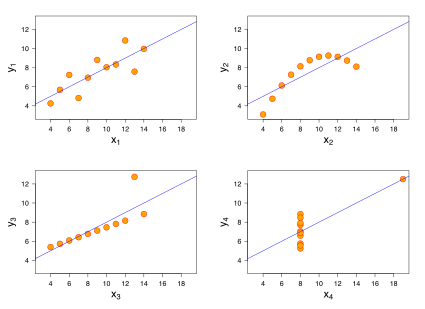
\includegraphics[width=0.8\textwidth]{./img/anscombie.png}    
  \end{center}
  
\end{frame}

\begin{frame}
  \frametitle{Ahora la regresión logística}

Asumimos que:
  \begin{align*}
    \mathcal{D} &= \{(x^{(1)}, y^{(1)}), \ldots, (x^{(M)}, y^{(M)})\} \\
    y &= h(x; w, b) + e, \quad x, w \in \mathbb{R}^n, b \in  \mathbb{R} \\
    y &= \sigma(x^T w + b) + e
    \end{align*}

    y asumimos que:
    $$
    y \sim \text{Bernoulli}(\rho) \ \text{i.i.d.}, \ \text{donde } \rho = \sigma(x^T w + b)
    $$
    y 
    $$
    \hat{y} = E[y | x; w, b] = \rho = \sigma(x^T w + b)
    $$
\end{frame}

\begin{frame}
  \frametitle{La receta secreta está en i.i.d.}

  Tenemos $\mathcal{D}$, un conjunto de datos i.i.d. de la variable aleatoria $y$.

  $$
  \Pr(y^{(1)}, \ldots, y^{(M)} | x^{(1)}, \ldots, x^{(M)}; w, b) = \prod_{i=1}^M \Pr(y^{(i)} | x^{(i)}; w, b)
  $$

  Los mejores valores de $w$ y $b$ son tales que:

  $$
  w^*, b^* = \arg \max_{w, b} \Pr(y^{(1)}, \ldots, y^{(M)} | x^{(1)}, \ldots, x^{(M)}; w, b)
  $$
\end{frame}

\begin{frame}
  \frametitle{Máximo de verosimilitud}
  $$
  w^*, b^* = \arg \max_{w, b} \prod_{i=1}^M \Pr(y^{(i)} | x^{(i)}; w, b)
  $$

  lo que nos lleva a maximizar el logaritmo de la verosimilitud:
  \begin{align*}
    w^*, b^* &= \arg \max_{w, b} \sum_{i=1}^M \log \Pr(y^{(i)} | x^{(i)}; w, b) \\
    &= \arg \max_{w, b} \sum_{i=1}^M \log \left|\rho^{y^{(i)}} (1 - \rho)^{1 - y^{(i)}}\right| 
  \end{align*}
\end{frame}

\begin{frame}
  \frametitle{Máximo de verosimilitud}
  \begin{align*}
    w^*, b^* &= \arg \max_{w, b} \sum_{i=1}^M \log \left|\rho^{y^{(i)}} (1 - \rho)^{1 - y^{(i)}}\right| \\
    &= \arg \max_{w, b} \sum_{i=1}^M y^{(i)} \log|\rho| + (1 - y^{(i)}) \log|1 - \rho| \\
    &= \arg \min_{w, b} \sum_{i=1}^M -y^{(i)} \log|\hat{y}^{(i)}| - (1 - y^{(i)}) \log|1 - \hat{y}^{(i)}| 
  \end{align*}
  que es la función de costo de la regresión logística de mínimo de entropía.
\end{frame}

\begin{frame}
  \frametitle{Aquí hay un patrón...}

  $$  
  \mathcal{D} = \{(x^{(1)}, y^{(1)}), \ldots, (x^{(M)}, y^{(M)})\} 
  $$
    
  y asumimos que:
  
  $$
  \Pr[y | x; w, b] = f(x^T w + b)
  $$

  y la estimación la hacemos encontrando:

  $$
  \hat{y} = E[y | x; w, b]
  $$
\end{frame}

\begin{frame}
  \frametitle{Familia exponencial de distribuciones}

  Una familia de distribuciones es exponencial si la función de densidad de probabilidad (o masa) se puede escribir como:
  $$
  \Pr[y; \eta] = f(y; \eta) = h(y) \exp(-A(\eta)) \exp(\eta^T T(y))
  $$
  donde:
  \begin{itemize}
    \item $h(y)$ es una función no negativa (medida de base)
    \item $A(\eta)$ es una función (\emph{función de partición})
    \item $\eta = (\eta_1, \ldots, \eta_n)$ son los parámetros naturales
    \item $T(x) = (T_1(x), \ldots, T_n(x))$ son las estadísticas suficientes
  \end{itemize}

  \begin{block}{}
    \emph{La familia exponencial es la familia de distribuciones más importante en estadística}
  \end{block}
\end{frame}

\begin{frame}
  \frametitle{La función de enlace (\emph{link function})}

  \begin{itemize}
    \item $\eta = (\eta_1, \ldots, \eta_n)$ son los parámetros naturales
    \item $\theta = (\theta_1, \ldots, \theta_n)$ son los parámetros de la distribución
    \item Existe una función $\phi$ tal que $\eta = \phi(\theta)$
    $$\eta = (\phi_1(\theta), \ldots, \phi_n(\theta))$$
    \item $\phi$ es la función de enlace
    \item $\phi^{-1}$ es la función de enlace inversa
  \end{itemize}
\end{frame}

\begin{frame}
  \frametitle{Ejemplo simple de la familia exponencial}

  Vamos a ver que pasa con $\mathcal{N}(\mu, \sigma^2)$, $\sigma$ fija
  
  \begin{align*}
    \Pr[y; \mu] &= \frac{1}{\sqrt{2 \pi \sigma^2}} \exp\left(-\frac{(y - \mu)^2}{2 \sigma^2}\right) \\
      &= \frac{1}{\sqrt{2 \pi \sigma^2}} \exp\left(-\frac{y^2 - 2 y \mu + \mu^2}{2 \sigma^2}\right) \\
      &= \frac{1}{\sqrt{2 \pi \sigma^2}} \exp\left(-\frac{y^2}{2 \sigma^2} + \frac{y \mu}{\sigma^2} - \frac{\mu^2}{2 \sigma^2}\right) \\
      &= \frac{1}{\sqrt{2 \pi \sigma^2}} \exp\left(-\frac{y^2}{2 \sigma^2}\right) \exp\left(\frac{y \mu}{\sigma^2} - \frac{\mu^2}{2 \sigma^2}\right) \\
      &= h(y) \exp(-A(\eta)) \exp(\eta^T T(y))
  \end{align*}  
\end{frame}

\begin{frame}
  \frametitle{continua ejemplo}

  Para este modelo, tenemos que:
  \begin{itemize}
    \item $h(y) = \frac{1}{\sqrt{2 \pi \sigma^2}}$
    \item $A(\eta) = \frac{\mu^2}{2 \sigma^2}$
    \item $\theta = \mu$
    \item $\eta = \frac{\mu}{\sigma^2}$
    \item $T(y) = y$
  \end{itemize}
  
\end{frame}

\begin{frame}
  \frametitle{Modelo lineal generalizado}

  Tenemos de evidencia:
  $$  
  \mathcal{D} = \{(x^{(1)}, y^{(1)}), \ldots, (x^{(M)}, y^{(M)})\} 
  $$ 
  y asumimos una distribución de la familia exponencial:
  $$
  \Pr[y | x; w, b] = f(y; \eta) = h(y) \exp(-A(\eta)) \exp(\eta^T T(y))
  $$
  donde:
  $$
  \eta = x^T w + b
  $$
  y la estimación la hacemos encontrando:
  $$
  \hat{y} = E[y | x; w, b]
  $$
\end{frame}

\begin{frame}
  \frametitle{Retomando la regresión logística}

  \begin{align*}
    \Pr[y | x; w, b] &= \text{Bernoulli}(\rho) \\
    &= \rho^{y} (1 - \rho)^{1 - y} \\
    &= \exp(y \log \rho + (1 - y) \log (1 - \rho)) \\
    &= \exp(y (\log \rho - \log (1 - \rho)) + \log (1 - \rho)) \\
    &= \exp(\log (1 - \rho)) \exp(y \log \frac{\rho}{1 - \rho}) \\
    &= h(y) \exp(-A(\eta)) \exp(\eta^T T(y))
  \end{align*}

\end{frame}

\begin{frame}
  \frametitle{Seguimos con la regresión logística}

  \begin{itemize}
    \item $h(y) = 1$
    \item $A(\eta) = -\log (1 - \rho)$
    \item $\theta = \rho$
    \item $\eta = \log \frac{\rho}{1 - \rho}$
    \item $T(y) = y$
  \end{itemize}

  Y sabemos que:
  \begin{itemize}
    \item $E[y | x; w, b] = \rho$
    \item $\eta = x^T w + b$
  \end{itemize}

  Por lo que:
  $$
  \hat{y} = E[y | x; w, b] = \rho = \frac{1}{1 + \exp(-(x^T w + b))}
  $$
\end{frame}

\begin{frame}
  \frametitle{¿Cuantas distribuciones son de la familia exponencial?}

  \begin{center}
    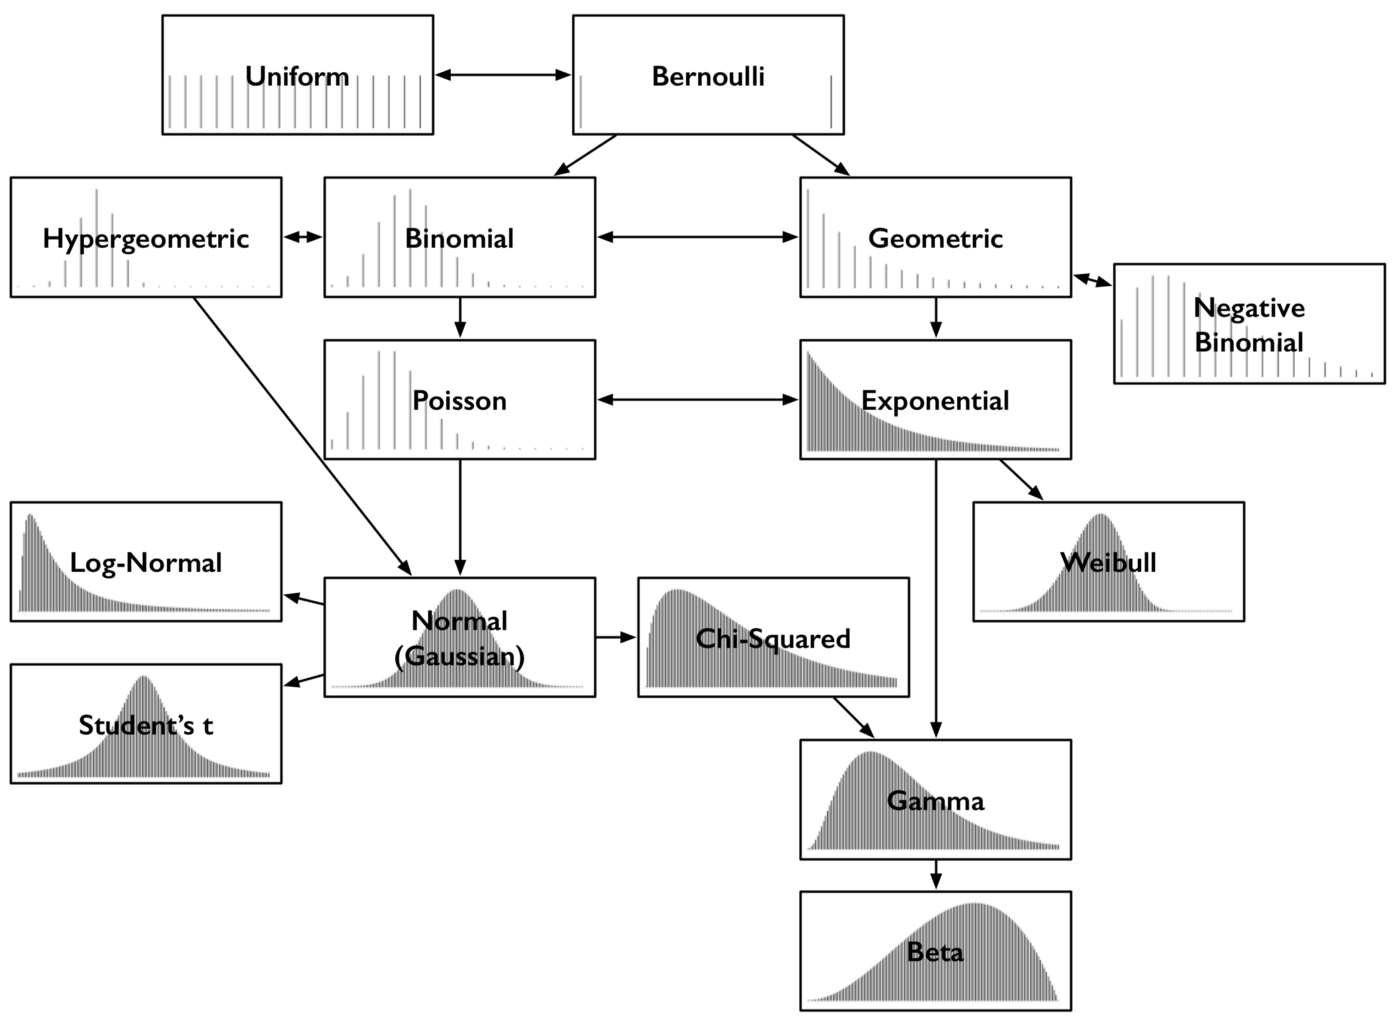
\includegraphics[width=0.8\textwidth]{./img/common_distributions.png}
  
    Algunas de ellas se pueden consultar en \href{https://en.wikipedia.org/wiki/Exponential_family\#Table_of_distributions}{Wikipedia}.
      
  \end{center}
\end{frame}

\begin{frame}
  \frametitle{Ejercicio}

  Si asumimos que tenemos $y \in \{p_1, \ldots, pk\}$ y consideramos un modelo lineal generalizado basado en una distribución categórica:
  \begin{itemize}
    \item ¿Cuales son los parámetros $\theta$?
    \item ¿Cuales son los parámetros naturales $\eta$?
    \item ¿Cual es la función de enlace y de enlace inversa?
    \item ¿Cuál es el vector de estadísticas suficientes $T(y)$?
    \item ¿Cual es el valor de $\hat{y}$?
    \item Deriva la función de costo usando máxima verosimilitud
  \end{itemize}

\end{frame}

\begin{frame}
  \frametitle{¿Y como los usamos en python?}

  \begin{itemize}
    \item Para regresión lineal, logística y categórica (softmax) es mejor usar los modelos de Scikit-Learn específicos.
    \item Scikit-Learn tiene una implementación de \href{https://scikit-learn.org/stable/modules/linear_model.html\#generalized-linear-models}{de modelos lineales generalizados}, aunque con pocas distribuciones (solo las \href{https://en.wikipedia.org/wiki/Tweedie_distribution}{distribuciones de la familia de Tweedie}).
    \item Statsmodels tiene una implementación más completa de \href{https://www.statsmodels.org/stable/glm.html}{modelos lineales generalizados}. Aunque es más compleja de usar, trata de parecerse a R.
    \item R no tiene competencia en este rubro. Si lo tuyo son los modelos estadísticos como los GLM con distribuciones extrañas, R es la solución.
  \end{itemize}
\end{frame}

\end{document}
